%%%%%%%%%%%%%%%%%% DOCUMENT SETUP %%%%%%%%%%%%%%%%%%

% Required IEEE parameters
\documentclass[letterpaper, 10pt, conference]{ieeeconf} % set document type
\IEEEoverridecommandlockouts                              % for \thanks command
%\overrideIEEEmargins                                      % use for \addtolength to normalize column lengths


% Packages
\usepackage{graphicx} % allows additional graphics formats
  \graphicspath{ {./images/} }
\usepackage{amsmath}   % assumes amsmath package installed
  \allowdisplaybreaks[1] % allow eqnarrays to break across pages
\usepackage{amssymb}   % assumes amsmath package installed 
\usepackage{url}       % format hyperlinks correctly
\usepackage{rotating}  % allow portrait figures and tables
\usepackage{subfigure} % allow matrices of figures
\usepackage{float}     % allows H option on floats to force here placement
\usepackage{multirow}  % allows merging of rows in tables
\usepackage{tabularx}  % allows fixed width tables
\usepackage{ctable}    % modifies \hline for use in table
\usepackage{bm}        % allow bold fonts in equations
\usepackage{wrapfig}   % allow text wrapping round figures
\usepackage{stfloats}  % control placement of floats
\usepackage[backend=biber,style=ieee,maxbibnames=3,bibencoding=utf8]{biblatex}   % allow bibliography control 
  \addbibresource{journal_abbreviations.bib}
  \addbibresource{references.bib}
\usepackage{siunitx}
\usepackage{placeins}

\usepackage{flushend}
% Custom commands
\newcommand{\matlab}{\emph{\sc{Matlab}}}
\newcommand{\maple}{\emph{\sc{Maple}}}
\newcommand{\simulink}{\emph{\sc{Simulink}}}
\newcommand{\dc}{d.c.}
\newcommand{\ac}{a.c.}
\newcommand{\rms}{RMS}
\newcommand{\wgn}{{\tt wgn}}
\newcommand{\sus}[1]{$^{\mbox{\scriptsize #1}}$}
\newcommand{\sub}[1]{$_{\mbox{\scriptsize #1}}$}
\newcommand{\chap}[1]{Chapter~\ref{#1}}
\newcommand{\sect}[1]{Section~\ref{#1}}
\newcommand{\fig}[1]{Fig.~\ref{#1}}
\newcommand{\tab}[1]{Table~\ref{#1}}
\newcommand{\equ}[1]{(\ref{#1})}
\newcommand{\appx}[1]{Appendix~\ref{#1}}
\newcommand{\degree}{\ensuremath{^\circ}}
\newcommand{\Vrms}{V\sub{\rms}}
\newcommand{\Vpp}{V\sub{pp}}
\newcommand{\otoprule}{\midrule[\heavyrulewidth]}         
\newcolumntype{Z}{>{\centering\arraybackslash}X}  % tabularx centered columns 


% Adjust figure spacing to get more text onto each page
\setlength{\abovecaptionskip}{1pt}
\setlength{\belowcaptionskip}{1pt}
\setlength{\dbltextfloatsep}{2pt}
\setlength{\dblfloatsep}{1pt}
\setlength{\floatsep}{1pt}
\setlength{\textfloatsep}{3pt}
%\addtolength{\skip\footins}{-10pt}


%%%%%%%%%%%%%%%%%% TITLE AND FRONT MATTER %%%%%%%%%%%%%%%%%%

% Title
\title{\LARGE \bf Design and implementation of a deep recurrent model for prediction of readmission in urgent care using electronic health records}

% Authors and affiliations 
%\author{Tahmina Zebin, Thierry J. Chaussalet, Shahadate Rezvy
%\thanks{T. Zebin and T.J. Chaussalet are with the School of Computer Science and Engineering, The University of Westminster, London, UK. Email: \tt{\small{\{zebint,chausst\}@westminster.ac.uk}}.}%
%\thanks{Middlesex University, London, UK. Email: \tt{\small{\{s.rezvy\}@mdx.ac.uk}}.}}%
%
\author{\IEEEauthorblockN{Tahmina Zebin,  Thierry J. Chaussalet }
\IEEEauthorblockA{School of Computer Science and Engineering,\\
University of Westminster, UK\\
Email: \{t.zebin, chausst\}@westminster.ac.uk}
%\and
%\IEEEauthorblockN{Shahadate Rezvy}
%\IEEEauthorblockA{Middlesex University, London, UK\\
%Email: {s.rezvy\@mdx.ac.uk}}
}


% Setup document 
\begin{document}
\maketitle
\thispagestyle{empty} % stop page numbers
\pagestyle{empty}


%%%%%%%%%%%%%%%%%% ABSTRACT %%%%%%%%%%%%%%%%%%
\begin{abstract}
There has been a steady growth in machine learning research in healthcare, however, progress is difficult to measure because of the use of different cohorts, task definitions and input variables. To take the advantage of the availability and value of digital health data, we aim to predict unplanned readmissions to the intensive care unit (ICU) from a publicly available Critical Care dataset called Medical Information Mart for Intensive Care (MIMIC-III). In this research, we formulate a heterogeneous LSTM and CNN architecture specifically to create a model of readmission risk. Our proposed predictive framework outperformed all the benchmark classifiers such as support vector machine, random forest and logistic regression models on all performance measures (AUC, accuracy and precision) except on recall where random forest  performed slightly better. Predictions from these models will help in resource planning and decrease mortality or length of stay in clinical care settings.
%We also propose an  weighted objective function combining individual task objectives. This loss function improves overall performance by ensuring that the model makes reasonable progress on all learning tasks. We demonstrate in experiments that the proposed multitask LSTM outperforms single-task baselines for the prediction tasks under consideration.


\end{abstract}
\begin{IEEEkeywords}
Deep learning; Electronic Health Records; Clinical Prediction; Readmission.

\end{IEEEkeywords}

%%%%%%%%%%%%%%%%%% INTRODUCTION %%%%%%%%%%%%%%%%%%
\section{Introduction} \label{sec:introduction}
Reducing costs, improving quality of care and effectively managing the resources are nowadays the main concerns of health-care decision makers \cite{curto2016predicting}. Traditionally models which predict in-hospital length of stay, readmission and mortality use the data available within the first 24 hours of admissions. Most of these models are designed to require as few inputs as possible and  focus on admission data and individual abnormal observations rather than patterns or trends over time \cite{tang2018predictive}. The emergence of machine learning to detect hidden patterns in complex, multi-dimensional datasets provides unparalleled opportunities to develop an efficient discharge decision-making support system for physicians. 
Deep learning models are well known for their end-to-end learning capabilities so we do not need to worry about the feature engineering part. Moreover, deep learning models are proved to be very powerful at distilling the complicated relationships hidden in the data and thus demonstrate good prediction performance. 
%https://www.biorxiv.org/content/biorxiv/early/2018/08/06/385518.full.pdf
In this research, we proposed supervised  deep machine learning approaches for ICU readmission prediction. In the intensive care unit (ICU), readmissions represent a type of adverse event that receives a lot of attention from the general medical community. Patients readmitted to the ICU have an increased risk of death. 
As such, it is of interest to keep patients in the ICU until such risk is minimal. Accurate prediction of hospital readmission can effectively help reduce the readmission risk (\fig{fig:readmission} shows exemplar transfers stages that happens in the ICU admission and readmission setting). However, the complex relationship between readmission and potential risk factors makes readmission prediction a difficult task. One of the main aims of this paper is to explore heterogeneous deep learning models to distill such complex relationships and make accurate predictions. The remainder of this paper is organized as follows. In \sect{sec:background} we present  MIMIC III ICU database\cite{johnson2016mimic}  and the current literature that has used deep learning models for clinical prediction tasks.  \sect{sec:methods} gives details for the implemented deep neural network architecture with the optional parameter settings and testing methods. We also provide various pre-processing and feature encoding stages for the readmission prediction task in this section and the classification results are shown in \sect{sec:results}. 
\begin{figure}
 \centering
 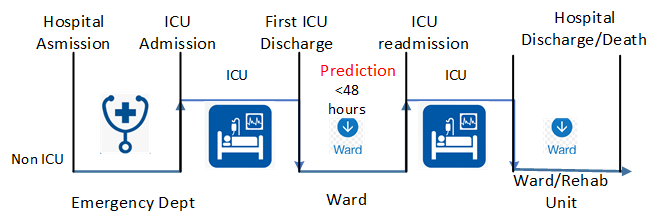
\includegraphics[width=0.49\textwidth]{Figures/mimic3.png}
 \caption{ Exemplar transfers undergone by an ICU patient. Since the patient’s first ICU stay was followed by another ICU stay, starting less than 48 hours later, these situations can be avoided by the readmission prediction.}
 \label{fig:readmission}
\end{figure}

%%%%%%%%%%%%%%%%%% BACKGROUND %%%%%%%%%%%%%%%%%%
\section{Background} \label{sec:background}

\subsection{Deep Learning for clinical predictions}
 
There is a good number of early research \cite{mobley2000predictions} that uses neural networks to predict  Length of stay (LOS) in hospitalized patients.  In our design, as we leveraged techniques from deep learning, here we call special attention to both historical and recent research that applies neural network architectures to clinical data or electronic health records. In predicting mortality from early admission data, feed forward neural networks nearly always outperform baselines based on logistic regression or severity of illness scores \cite{clermont2001predicting}. Machine learning techniques like state space models and time series mining to integrate more detailed data about the patient into mortality prediction have also been used in the literature. Recently, novel deep learning architectures have been proposed for survival analysis \cite{ranganath2016deep}. Many of these works aim to make predictions based on complex temporal patterns of physiology rather than individual patient measurements. Others leverage information from clinical notes, extracted using topic models \cite{lipton2015learning}. However, the results are generally not comparable due to use of different data, hence we attempted to develop our models using a publicly available dataset described in the next subsection.

\subsection{MIMIC-III Dataset}
Medical Information Mart for Intensive Care III (MIMIC-III) is a database comprising Electronic Health Record (EHR) information related to patients admitted to critical care units at the Beth Israel Deaconess Medical Centre, in Boston, USA. MIMIC-III consists of the health-related EHR data of more than 40,000 patients between 2001 and 2012. It contains data such as: vital signs, medications, laboratory measurements from within the hospital (i.e. in-patient) and from clinics (i.e. out-patient), charted observations during a patient’s stay in the intensive care unit, and de-identified notes regarding the patient’s stay, including nursing notes, physician notes and discharge summaries \cite{johnson2016mimic}. MIMIC-III consists of 26 relational tables, where 16 of them contain timestamped event information. Tables are linked by identifiers: $SUBJECT\_ID$ refers to a unique patient and $HADM\_ID$ refers to a unique admission. For this study, we have mainly used chartevents table, along with linked $d\_item$ table to get the label of $item_id$ specified in the chartevents table. Diseases and procedures in the MIMIC-III are encoded using the International Classification of Diseases version 9 (ICD-9) codes, and the mapping can be found in $diagnoses\_icd$ and $procedures\_icd$ tables. Time in the MIMIC-III database is stored with one of two suffixes: TIME (down to the minute) and DATE (down to the day). Most data are recorded with a time indicating when the event took place (CHARTTIME) and when it was validated (STORETIME). In this research, the event logs were created using CHARTTIME attributes, as this is the best match to the time of actual measurement. All the patient data in the MIMIC-III database has been de-identified and all dates have been randomly shifted to the future so that dates are internally consistent for the same patient but inconsistent across patients \cite{Desautelse017199}.

\subsection{ Patient Screening for readmission modelling}

We processed the MIMIC-III dataset to construct a representative readmission dataset where we first screened out the patients under age 18, and have removed the patients who died in the ICU. This results in total 35,334 patients with 48,393 ICU stays. To be noted, one patient may have multiple in-hospital records in the dataset. We then split the processed patients into training(80\%),
validation(10\%)and testing(10\%) partitions and conduct a five-fold cross validation. In the ICU readmission dataset, we categorized all selected patients and the corresponding ICU stay records into positive or negative cases. Positive cases are regarded as ones in which the patients could benefit from a prediction of readmission before being transferred or discharged. Negative cases, on the 
contrast, are those that the patient do not need ICU readmission. Specifically, patients who were transferred or discharged from ICU and did not return and are still alive within the next 30 days are considered to be negative cases \cite{Desautelse017199}. In the MIMIC Dataset, we had the following instances that contributed to the positive cases: i) patients were transferred to low-level wards from ICU, but returned to ICU again (3,555 records); ii) patients were transferred to low-level wards from ICU, and died later(1,974 records); iii) patients were discharged, but returned to the ICU within the next 30 days (3,205 records); iv) patients were discharged, and died within the next 30 days (2,556 records). \fig{fig:exp} illustrates the patient age distribution and readmission count by days for the the discussed patient groups.


\begin{figure*}
  \centering
  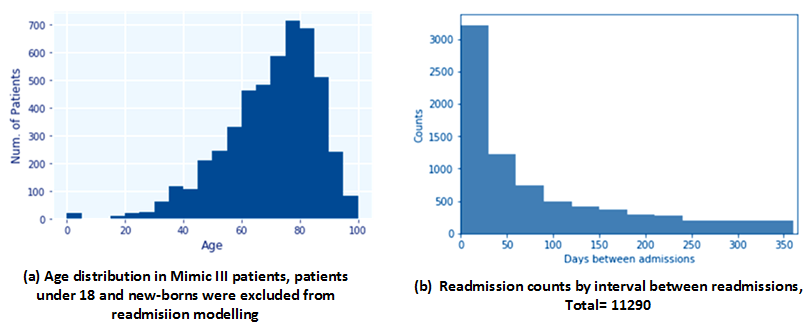
\includegraphics[width=0.78\textwidth]{Figures/mimic3_readmission_exploratory.png}
\caption{Exploratory Analysis for readmission modelling. (a) Age distribution; (b) Readmission count by days }
\label{fig:exp}
\end{figure*}

%we want to predict UNPLANNED re-admissions, so we should filter out the ELECTIVE next admissions.
%the NEWBORN admissions were missing discharge summaries vs ~4% for the others. At this point I decided to remove the NEWBORN admissions. Most likely, these missing NEWBORN admissions have their discharge summary stored outside of the MIMIC dataset.

\subsection{Dealing with the data imbalance}
The dataset for the readmission modelling task was relatively imbalanced, with the positive group that went through any form of readmission formed of 11290 instances out of 48393 ICU stays. This resulted in a positive and negative readmission class ratio of 1:3.3.  The machine learning literature proposes to handle data imbalance through either under-sampling or over-sampling strategies. The former involves reducing the majority class by the removal of instances from the training set, while the latter over-samples with repetition from the minority class, thus increasing its impact within the training process. Several variations of under- or over-sampling were proposed in previous studies, including the one-sided selection and Synthetic Minority Oversampling Technique (SMOTE) \cite{witten2016data}. We have applied the latter on the training dataset to avoid any bias during the training stage.

\subsection{ 48 hour chart event segmentation}

For temporal information modeling of the time-series ICU records, a 48-hour window on each ICU stay has been applied. From literature it was observed that, the data during the last 48 hours before the patient is discharged or transferred to a lower level ward are the most informative for readmission 
prediction. Therefore, we separated out last 48-hour data from each ICU record for the modelling purpose. To maintain consistency, if a record was found shorter than 48 hours, we replicated the data of the last hour to fill the gap in the 48 hour record window. 


 %\begin{figure}
%    \centering
%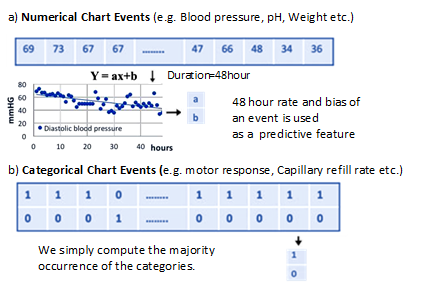
\includegraphics[width=0.49\textwidth]{Figures/mimic3_4.png}
%\caption{Statistical feature computation procedure for numerical chart events and categorical events}
% \label{fig:stat}
 % \end{figure}

%https://towardsdatascience.com/introduction-to-clinical-natural-language-processing-predicting-hospital-readmission-with-1736d52bc709



%we will make use of the following MIMIC III tables

%ADMISSIONS:a table containing admission and discharge dates (has a unique identifier HADM ID for each admission)
%NOTEEVENTS: contains all notes for each hospitalization (links with HADM ID)



%%%%%%%%%%%%%%%%%% METHODS %%%%%%%%%%%%%%%%%%

%    \begin{figure*}
 %     \centering
      %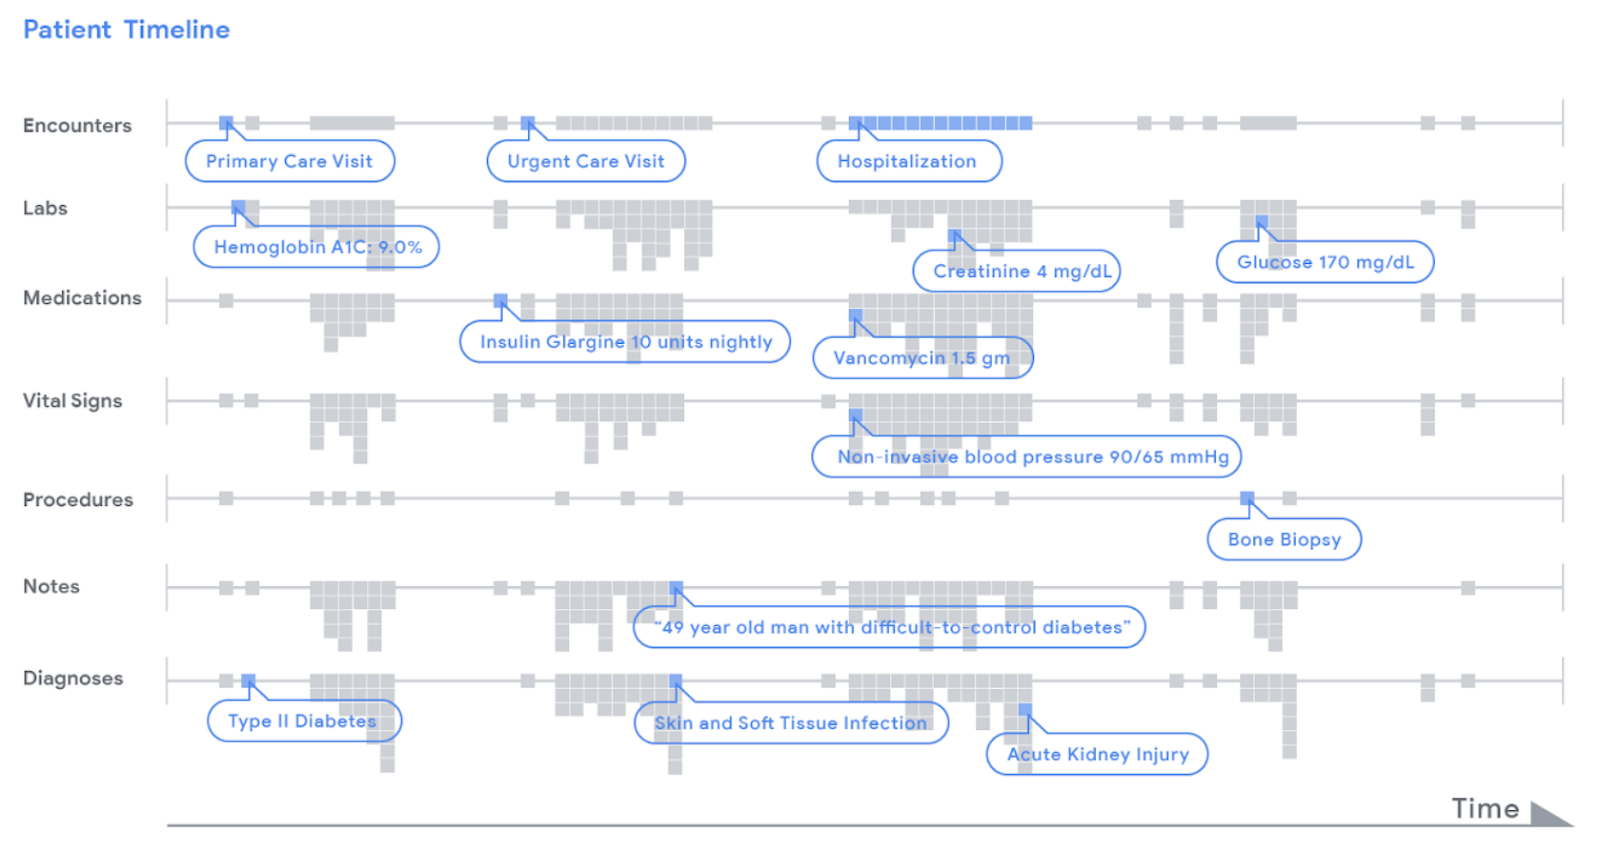
\includegraphics[width=0.95\textwidth]{Figures/image3.png}
 %     \caption{An example segment of electronic health records, with vital signs, medications, procedure and diagnosis are recorded at different encounters at primary care, urgent care and hospitalization }
 %     \label{fig:workflow}
%    \end{figure*}


\section{Readmission Modelling}\label{sec:methods}
In this section, we provide a brief description of the proposed model along with the demographics, disease code and chart events features used in  our ICU readmission modelling tasks from MIMIC III dataset. As readmission modelling uses time series data, we attempted multiple model structures including bidirectional LSTM, CNN, and various combinations of them to automate the feature extraction process. The mathematical foundation for LSTM can be found in ref \cite{zebin2018human,lin2018analysis}. After exploring the models systematically, we finally proposed a heterogeneous LSTM+CNN model, where the CNN computes the feature maps without zero padding after receiving the output hidden unit sequence from LSTM. 

\subsection{Model Architecture}

A summary of the  proposed LSTM+CNN model architecture is shown in \fig{fig:lstm}. We have utilized the \emph{sequential} model and the \emph{dense}, \emph{Conv1D}, \emph{LSTM}, \emph{concetenate}, and \emph{batch normalization} layers from the python keras toolbox. 

At the very first layer, we fed the  processed chart events in 48-h structured windows, along with encoded demographic features and ICD-9 embedding features to build up internal states of the bidirectional LSTM layer and update its weights to generate the significant memory states in the data.
The learning rate of training was set to $1\times 10^{-3}$, and we used binary cross-entropy along with an Adam optimizer (beta =0.9) during the training stage of the model.
After that the CNN layer receives the output sequence from final bidirectional  LSTM layer and computes the feature maps to be fed to the output decision making layer.
We have used a softmax activation function as the output dense decision layer. The layer calculates the loss between the predicted values and the true values, and the weights in the network are adjusted according to the loss. Our proposed classification model was implemented using python keras library \cite{keras} with TensorFlow back end. All of our evaluations were performed on a linux pc with an Intel Xeon 3.60GHz processor, 128 GB RAM and an NVIDIA Titan V GPU. 

\begin{figure}
    \centering
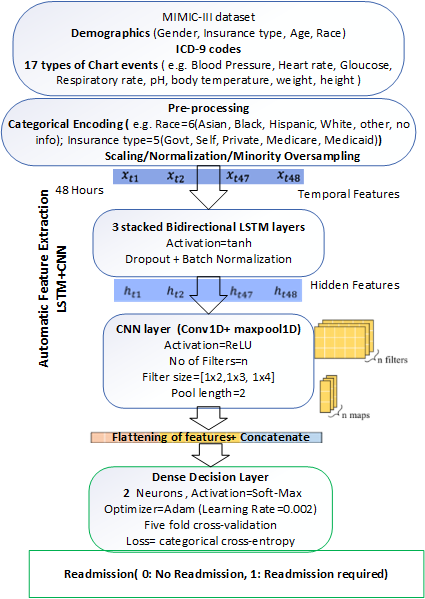
\includegraphics[width=0.45\textwidth]{Figures/mimic3_readmission.png}
\caption{LSTM+CNN model, and CNN computes the feature maps for final classification after receiving the output hidden unit sequence from LSTM.}
\label{fig:lstm}
  \end{figure}   

 \begin{table*}[h!]
\centering
\caption{Quantitative comparison of  LSTM+CNN with other traditional classifications.}   \label{table:performance_comparison}
 \begin{tabularx}{0.96\textwidth}{X Xcccc}
    \toprule
    Classifier & Features&  Acuracy (\%)& Precision(\%)& Recall (\%)& Area Under Curve (AUC) \\
    \otoprule
     Statistical Models:
     Logistic Regression & CE STAT + ICD-9+ D &  70.3 & 87.2& 73.6& 0.714 \\
     Random Forest & CE STAT + ICD-9+ D &  72.3 & 89.2& 75.6 & 0.770 \\
     Support Vector Machine & CE STAT + ICD-9 +D &  71.1 & 90.4& 72.2 & 0.775 \\
     \midrule
     LSTM & 48-h CE only &  69.5 & 89.4& 68.6& 0.761\\
     LSTM & 48-h CE+ ICD-9 + D &  70.7 & 90.6& 73.3 & 0.787\\
     LSTM+CNN & 48-h CE+ ICD-9 + D &  73.1 & 92.2& 74.2 & 0.821\\
     
    \bottomrule
  \end{tabularx}
\end{table*}
 
 \subsection{Chart Events, demographics and ICD-9 features}
   
There are several significant groups of variables for predicting readmission. The first 
group of variables are chart events. Chart events are recorded from notes of healthcare providers (e.g., physicians and nurses) and represent the patients’ physiological conditions from experts’ observation and opinions \cite{XUE2018}.  Second, patient variables, especially chronic diseases, that are found strongly associated with ICU readmission risk \cite{Brown2013}. Thirdly, the basic demographic information, such as gender, age, race, that are again demonstrated as important factors in the state of art readmission prediction . The demographic features we consider consist of the patients’ gender, age, race, and insurance type. The reason for including insurance type (uninsured) could lead to insufficient payment and might result in an unexpected discharge. The whole dimension is fourteen for the four demographic features we considered in this study.
Chronic diseases are one of the most important factors associated with later readmissions. To deal with the EHR ICD-9 codes, we regrouped them in 17 broad classes. For this study, our features consist of 17
chart events (e.g. weight, height, pH, respiratory rate, body temperature, systolic and diastolic blood pressure, capillary refill rate, Glascow coma eye, verbal and motor response parameters) are encoded in 59 channels, 17 diagnoses code groups, and 14 channels for demographic information of the patients. 

\subsection{Statistical features}
To compare the proposed model with some traditional methods like logistic regression, we also extract statistical features from the chart events for usage \cite{lin2018analysis}.
For the implementation of the traditional methods, we also extract the statistical features within each 48-hour window. For the numerical chart events such as diastolic blood pressure or pH, we regress the 48 data points from the 48 hour window linearly and record the rate and the bias in the linear function. For categorical events 
(e.g. motor response, capillary refill rate), we simply compute the majority occurrence of the event in that category.

%%%%%%%%%%%%%%%%%% RESULTS %%%%%%%%%%%%%%%%%%
\section{Results and Discussion} \label{sec:results}

 In this section, we evaluated the performance of the modelwith traditional statistical approaches such as logistic regression, random forest etc, and variants of deep leaning models such as Long-Short Term Memory(LSTM) and Convolutional Neural Networks (CNN). We compared the performance obtained by different models and derived the optimal solution of the prediction system. 
 For the proposed LSTM+CNN model, CNN computes the feature maps without zero padding after receiving the output hidden unit sequence from LSTM. Our experimental results showed that LSTM followed by a CNN utilizing all the feature sets obtains a higher positive recall rate and overall prediction performance. The proposed model outperforms the traditional approaches trained with statistical features. 
 %The ROC curve of some selected models and features are shown in \fig{fig:roc}. 
 Our experiment results showed that LSTM followed by a CNN utilizing all the feature sets obtains a
higher positive recall rate and better prediction performance than its generic LSTM counterpart to explore temporal relationship in the data. As can be seen in \tab{table:performance_comparison}, we also experimented with various combination of available feature sets to train variants of LSTM. The proposed model with the full feature set outperforms the traditional approaches trained with statistical features and selective raw features from the chart events, ICD-9 embeddings and the demographic features. 

The LSTM trained with basic 48 hour chart events (shown in green in \fig{fig:roc})  had an area under the curve (AUC) value of 0.76 while with the proposed LSTM+CNN (shown in purple) with added demographics and ICD-9 embeddings acheived higher AUC value of 0.821. Though the implemented deep learning models take longer to train and to extract the automated features than the statistical models, they are able to predict faster due to the absence of manual feature calculation stage.

\begin{figure}[h!]
  \centering
  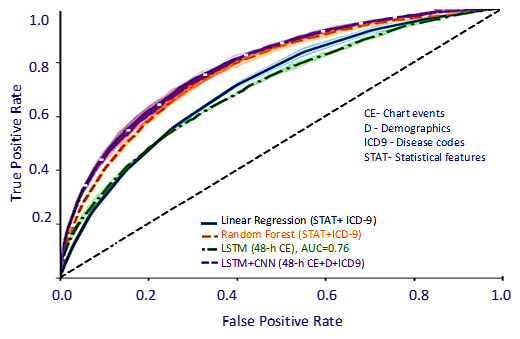
\includegraphics[width=0.40\textwidth]{Figures/mimic3_RoC.png}
\caption{ROC curve of some of the attempted models and features. The color bar is the error bar of the ROC curve with five-fold cross validation. LSTM-CNN model performs relatively better than random forest, logistic regression and the generic LSTM model. }
\label{fig:roc}
\end{figure}




% \begin{figure*}[h!]
%    \centering
%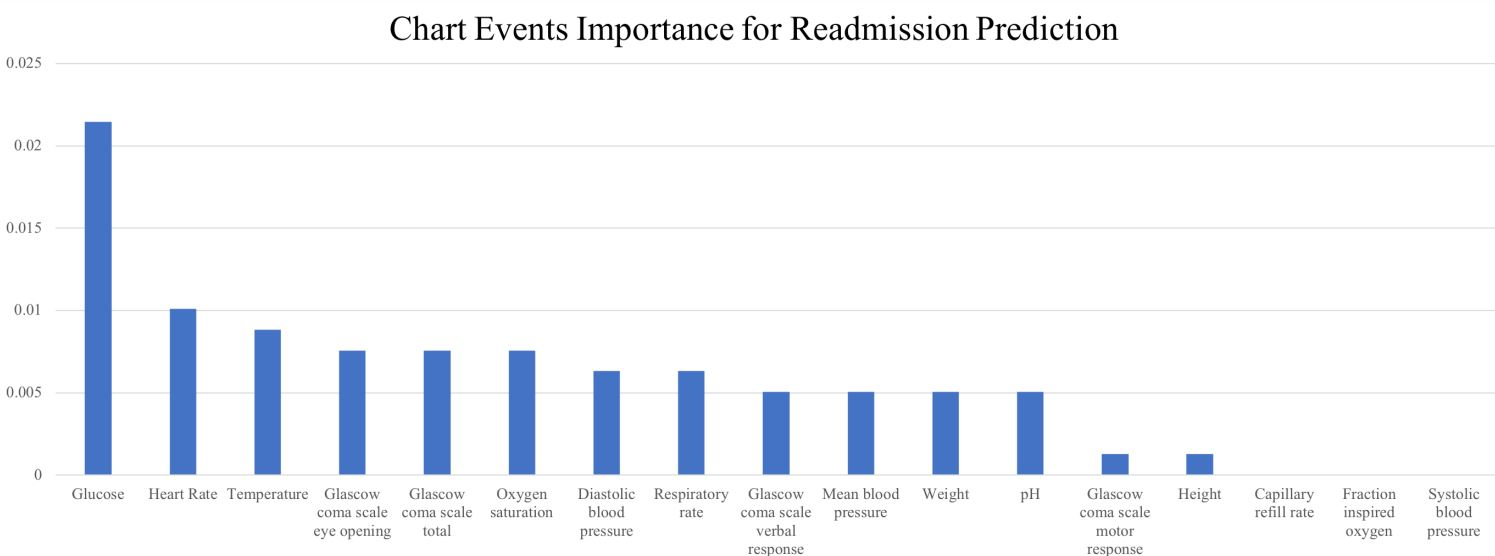
\includegraphics[width=0.95\textwidth]{Figures/chart_events.JPG}
%\caption{The ranking of chart events accordint to importance when predicting the ICU readmission. }
%\label{fig:rank}
 % \end{figure*}

 
%%%%%%%%%%%%%%%%%% CONCLUSIONS %%%%%%%%%%%%%%%%%%
\section{CONCLUSIONS} \label{sec:conclusions}

 We leveraged the MIMIC-III dataset to provide clinicians with data-driven decision-making support that can help to prevent inappropriate discharge or transfer of patients that are high-risk for readmission so that ICU can reduce effectively the risk to the patient of readmission and reduce cost. The proposed  models  presented in this research may find application either in helping with ICU discharge decisions, or in better targeting ward resources towards patients with a high chance of unplanned readmission before any adversity or harm can occur. The proposed predictive framework showed quantitatively superior performance (73.1\% ) to that of the benchmark statistical predictors such as SVM (Accuracy: 71.1\%), random forest (Accuracy:72.2\%) and logistic regression models (Accuracy:70.3\%) in terms of model accuracy. In the future, we will extend our models to provide higher overall accuracy in multi-task clinical prediction problems \cite{harutyunyan2017multitask}.

%%%%%%%%%%%%%%%%%% REFERENCES %%%%%%%%%%%%%%%%%%

%\FloatBarrier
\section*{Acknowledgement}
We gratefully acknowledge the support of NVIDIA Corporation with the donation of the Titan V GPU and the Quintin Hogg Trust for funding this work through the Health Innovation Ecosystem at the University of Westminster.

\renewcommand*{\bibfont}{\small}

\printbibliography


\end{document}
